% The command to run latex:
%   pdflatex report
%
% The command to run the bibtex:
%   bibtex report

\documentclass[pdftex,twoside,a4paper]{report}

\usepackage[pdftex]{graphicx}
\usepackage[margin=3.0cm]{geometry}
\usepackage[english]{babel}
\usepackage[normalem]{ulem}
\usepackage{algorithm2e}
\usepackage{amsfonts}
\usepackage{amsmath}
\usepackage{amssymb}
\usepackage{tabularx}
\usepackage{color}
\usepackage{tabto}
\usepackage{graphicx}
\usepackage{hyperref}
\newcommand{\hilight}[1]{\colorbox{yellow}{#1}}
\newcommand{\TODO}{\hilight{NOT DONE}}
\newcommand{\hs}{$\hspace{0.5cm}$}
\newcommand{\bt}{\begin{tabbing}}
\newcommand{\et}{\end{tabbing}}
\newcommand{\bcen}{\begin{center}}
\newcommand{\ecen}{\end{center}}
\newcommand{\length}{\ell}
\newcommand{\pmem}{Particle Mesh Ewald method}
\newcommand{\fma}{Fast Multipole Algorithm}

\begin{document}

\begin{titlepage}
 
\begin{center}


\includegraphics[width=0.8\textwidth]{logoWhite.png}\\[0.5cm]
\textsc{\Large School of Computer Science}\\[0.5cm]
\textsc{\Large College of Engineering and}\\[0.2cm]
\textsc{\Large Computer Science}\\[0.5cm]


 
\vspace{1.4cm}

\hrule

\vspace{1.4cm}

{ \huge \bfseries The Fast Multipole Algorithm vs the Particle Mesh Ewald method} \\

\vspace{0.4cm}

{ \LARGE \bfseries Joshua \textsc{Nelson} - u4850020} \\

\vspace{1.4cm}


\hrule

\vspace{1.0cm}

\textsc{\large COMP3006 - Computer Science Research Project}\\

\vspace{1.0cm}

\hrule

\vspace{1.4cm}



\emph{Supervisor: } 
Dr Eric \textsc{McCreath} \\

 
\vfill
 
% Bottom of the page
{\large \today}
 
\end{center}
 
\end{titlepage}



\begin{abstract}
The N body problem is common across the fields of physics, biology and chemistry. The classic solution to this problem has an inhibitive complexity in the class $O(n^2)$. Two alternative methods were examined: The Fast Multipole Algorithm, and the Particle Mesh Ewald Method, with better complexities of $O(n)$ and $O(n \text{log}(n))$, respectively. These algorithms were implemented in Java, and their efficiencies were discussed and compared. The algorithms were run over typical molecular dynamics simulations to determine the most efficient algorithm for the N-body problem.
\end{abstract}

\tableofcontents

%_____________INTRODUCTION CHAPTER________________
\chapter{Introduction}
\section{The N body problem}
    Suppose we have a collection of $n$ bodies in some space, that interact with each other. Each body interacts with every other body in the system in a pairwise way. Often this pairwise interaction is a function of the distance between the bodies, and their properties, such as mass or electric charge. The task is to calculate the total effect on each body from every other body.\\
    
    The N body problem is key to the simulation of many different scientific environments. The bodies may be astrophysical objects, such as planets or galaxies, interacting based on distance and body mass \cite{MilleniumRun}, or atoms in a molecular dynamics simulation, based on distance and particle charge.\cite{NAMD}. For the remainder of the report, we will discuss the N body problem in regards to Molecular dynamics, however the approaches can be generalised.
    
\chapter{Algorithms for the n body problem}
\section{The $O(n^2)$ solution}
        
%%%%%%%%FIGURE%%%%%%%%%%%%%
\begin{figure}[h]
\bcen 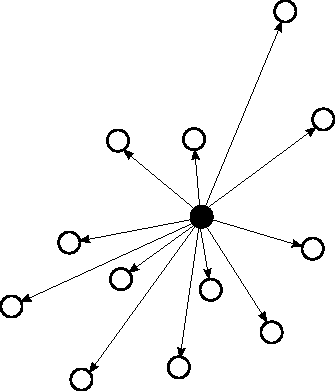
\includegraphics{figures/nbodies.pdf} \ecen
\caption{The na\"{\i}ve approach to the n body problem - calculate each interaction for each particle}
\end{figure}

The simplest solution to the N body problem is the basic $O(n^2)$ approach of calculating each interaction directly. Pseudocode for the algorithm is given below.\\

%%%%%PSEUDOCODE%%%%%%%%%
\begin{algorithm}[H]
 \SetLine
 \KwData{$r_i$: particle positions, $q_i$: particle charges, N: number of particles, Q: output array of charges}
 \For{i=0 to N}{
  \For{j=i to N}{
      \If{$i \not= j$}{
        $d := |r_i - r_j|$\;
        $Q[i] := q_i * q_j / d$\;
       }
  }
 }
 \caption{The basic approach to the N body problem}
\end{algorithm}

The advantages to the $O(n^2)$ approach are it's simplicity, ease of implementation, and it's low overhead. However, it's primary disadvantage is that it is limited to small numbers of particles by it's $O(n^2)$ complexity. These advantages and disadvantages are further discussed in Chapter \ref{chap:compare}


\section{The particle mesh ewald method}
\subsection{Background}
\subsubsection{Ewald summation}
The key concept behind the \pmem is that of \emph{Ewald Summation}. Ewald Summation splits the potential between two particles into two components, the long range force and the short range force. \cite{petersen:3668}
\[
\phi(r) = \phi_{\text{sr}}(r) + \phi_{\text{lr}}(r)
\]
The advantage of doing this is that $\phi_{\text{sr}}$, the short range term, can be converges quickly in real space, while $\phi_{\text{lr}}$ converges quickly in reciprocal space. The \pmem takes advantage of this by calculating the $\phi_{\text{sr}}$ term by calculating potential directly for nearby particles, and uses a grid based direct fourier transformation to calculate the long range component.
\subsubsection{Real space computation}
The short range potential at a point can be computed by considering only particles within a small radius of the point. We can keep the radius small as $\phi_{\text{sr}}$ converges quickly in real space. This is also important, as we need to keep the number of particles considered less than $N$, in order to reduce the algorithm from $O(n^2)$ complexity. This is the case though, as the radius we consider is constant and less than the size of the simulation cell width, and we assume the particles are distributed randomly within the simulation cell.
%%%%%%%%FIGURE%%%%%%%%%%%%%
\begin{figure}[h]
\bcen 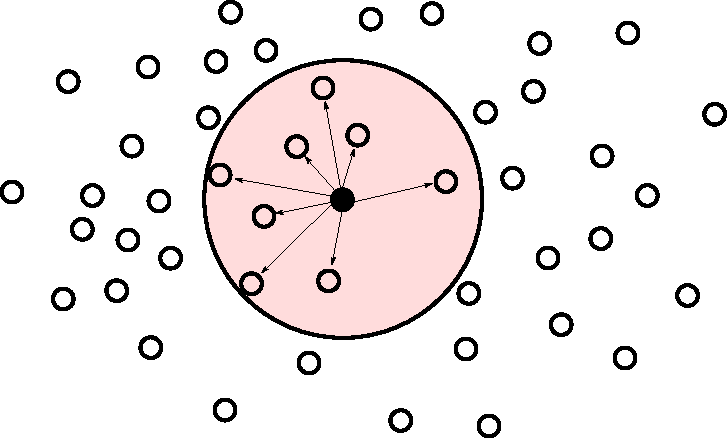
\includegraphics{figures/cutoff.pdf} \ecen
\caption{A particle and the particles that we consider it's interactions with, based on the cutoff distance}
\end{figure}

\subsubsection{Reciprocal space computation}
The reciprocal space is the long range part of the potential computation, and which converges slowly in real space. However, in reciprocal space, it converges quickly, so we use discrete fourier transformations to calculate this part of the sum.\\

Discrete fourier transformations require a discrete space to transform, however, our real space is continuous. So for this, we need to discretise the charges onto a grid. The approach taken in the original paper was to use Lagrangian interpolation to achieve this. Close mesh cells receive most of the charge from each particle, and this amount decreases to zero at some point, depending on the interpolation order. This is described in detail in Section \ref{sec:math_desc_lagrange}.\\
%%%%%%%%FIGURE%%%%%%%%%%%%%
\begin{figure}[h]
\bcen 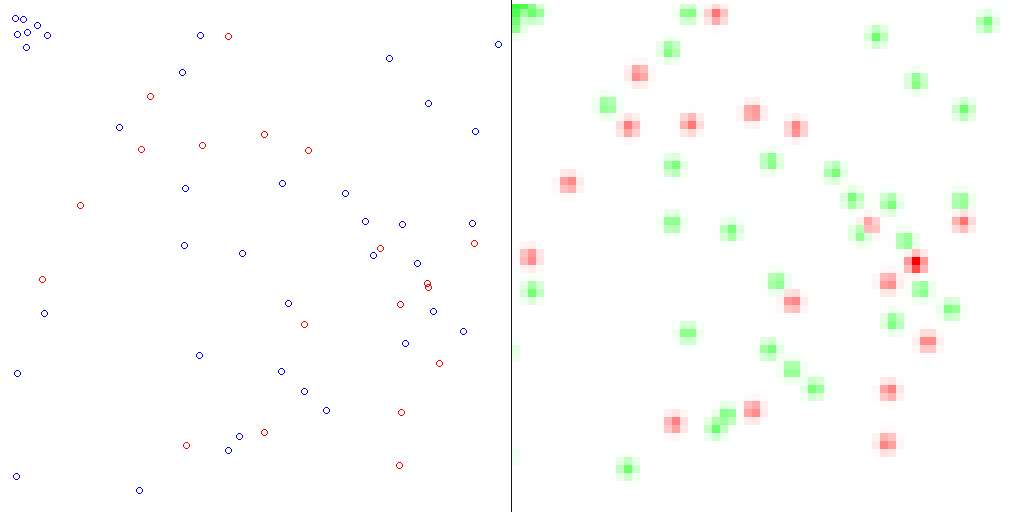
\includegraphics[width=\textwidth]{figures/Qarray.jpg} \ecen
\caption{A distribution of continuous charges, and an interpretation of them as discrete charges}
\end{figure}

An alternative to using lagrange interpolation is to use cardinal B splines. This modification is known as the \emph{Smooth Particle Mesh Ewald} method, and is advantageous in terms of accuracy, and is also easily differentiable, which is important if the forces are required as well as the potentials.  \cite{essmann:8577} This is the method that was implemented in this paper.

\subsection{Mathematical description}
\subsubsection{Interpolating the charges to the Q array}
\label{sec:math_desc_lagrange}
We first present the formulation of the Q array based on lagrangian interpolation. 
\begin{equation} \label{eq:q_array}
Q(k_1,k_2) = \sum_{i=1} ^N \sum_{n_x,n_y} q_i W_{2p}(u_{xi} - k_1 - n_xK) * W_{2p}(u_{yi} - k_y - n_yK)
\end{equation}
Where $N$ is the number of particles,\\
$n_1,n_2$ are integers $< N$,\\
$W_{2p}$ is a Lagrangian polynomial of order $p$ with a value in the range $[0,1]$,\\
$K$ is the number of cells we split the grid into,\\
$u_{xi}, u_{yi}$ are scaled fractional coordinates of particle $i$ (Scaled fractional coordinate coordinates meaning $u_{xi} = K * (r_{xi} / (\text{simulation width}))$, $r_{xi}$ is the particle i's $x$ coordiante, so $0 \leq u_{xi} \leq K$).\\
More information can be found in \cite{essmann:8577}\\

We can replace $W_{2p}$ in the above with $M_n$, a cardinal B spline of order $n$, and the formulation of the Q array is the same. From this point forward, we will use cardinal B spline interpolation.
\subsubsection{Calculating electrostatic potential from the Q array}
With this Q array we can long range contribution to the electrostatic potential in reciprocal space.\\
The reciprocal space contribution to the electrostatic energy can be written as,\\
\begin{equation}
E_{\text{rec}} = \frac{1}{2*\pi*V} \sum_{m \not= 0} \frac{\text{exp}(- \pi^2 m^2 / \beta^2)}{m^2} B(m_1,m_2) S(m) S(-m)
  \label{eq:primitive_rec_energy} \end{equation}
Where $V$ is the volume (or in the two dimensional case, area) of the simulation cell,\\
$\beta$ is the ewald coefficient,\\
$S$ is the structure factor.\\
$B$ is the matrix of B spline inverse fourier transform moduli, $B(m_1,m_2) = |b_1(m_1)|^2 * |b_2(m_2)|^2$. More detail on this can be found in \cite{essmann:8577}.\\
It is shown in \cite{essmann:8577} that $S(m) \approx F(Q(m))$, so we can rewrite this as a convolution\\
\begin{equation}
E_{\text{rec}} = \frac{1}{2} \sum_{m_1 = 0}^K \sum_{m_2 = 0}^K Q(m_1,m_2) * (\theta_{\text{rec}} \star Q)(m_1,m_2)
\label{eq:energy_rec}
\end{equation}
With $\theta_{\text{rec}} = F(B * C)$, and so $(\theta_{\text{rec}} \star Q)(m_1,m_2) = F(B * C * F^{-1}(Q))$ \cite{essmann:8577} \cite{lee05}\\
Where $C$ is the matrix for the original exponential term from Equation \ref{eq:primitive_rec_energy}, that is,
 \bcen$\displaystyle
C(m_1,m_2) = \frac{1}{\pi V} \frac{\text{exp}(- \pi^2 m^2 / \beta^2)}{m^2} $ for $ m \not= 0, C(0,0) = 0
$\ecen 
\subsubsection{The ewald coefficient}
The ewald coefficient, $\beta$, is a number describing the ratio between the real space and the reciprocal space contributions to the calculation of the total energy. In practice, it depends on the tolerance $\epsilon_\text{tol}$, and our desired cutoff distance $r_{\text{cut}}$ in the following way, \cite{darden:10089} \cite{essmann:8577}\\
\begin{equation}
\frac{\text{erfc}(\beta r_{\text{cut}})}{r_\text{cut}} \leq \epsilon_\text{tol}
\label{eq:ewald_coeff}
\end{equation}
Where erfc is the complimentary error function, a function that tends quickly to zero, depending on it's argument. The relation means that for $r > r_{cut}$, we have $\frac{\text{erfc}(\beta r_{\text{cut}})}{r_\text{cut}} \leq \epsilon_\text{tol}$, and for all $r > r_\text{cut}$ we can ignore the direct energy contribution, given by equation \ref{eq:energy_dir} \cite{essmann:8577}\\
\begin{equation}
E_\text{dir} = \frac{1}{2} \sum_{n} \sum_{i,j = 1} ^N \frac{q_i q_j \text{erfc}{\beta |r_j - r_i|}}{|r_j - r_i|}
\label{eq:energy_dir}
\end{equation}
Which becomes
\begin{equation}
E_\text{dir} = \frac{1}{2} \sum_{n} \sum_{i,j = 1} ^{\overset{*}{N}} \frac{q_i q_j}{|r_j - r_i|}
\label{eq:energy_dir_noerfc}
\end{equation}
Where the $*$ indicates terms with $|r_j - r_i| > r_{\text{cut}}$ are left out of the sum
\subsection{The algorithm}
\subsubsection{Main particle mesh ewald flow}
The basic flow of the algorithm is given below\\ \newline
%%%%%PSEUDOCODE%%%%%%%%%
\begin{algorithm}[H]
\SetLine
Initialise the ewald coefficient (Equation \ref{eq:ewald_coeff})\\
Calculate the B spline coefficients (Details in \cite{essmann:8577})\\
Allocate particles to their cells (Section \ref{sec:verlet})\\
Initialise the Q matrix (Equation \ref{eq:q_array})\\
Calculate reciprocal energy (Equation \ref{eq:energy_rec})\\
Calculate direct energy (Equation \ref{eq:energy_dir})\\
\end{algorithm}

\subsubsection{Verlet list algorithm}
\label{sec:verlet}
The following algorithm utilises a list known as a \emph{Verlet list} to keep track of which particles are within a cutoff distance of each other, with only $O(n)$ complexity. It is used in the direct energy calculation of the \pmem\\
%%%%%PSEUDOCODE%%%%%%%%%
\begin{algorithm}[H]
\SetLine
\For{i=0 to N}{
    $\text{cell}_x := \lceil u_{xi} \rceil$; (With $u_{xi}$ the scaled fractional x coordinate, as defined in Equation \ref{eq:q_array}))\\
    $\text{cell}_y := \lceil u_{yi} \rceil$; (With $u_{yi}$ the scaled fractional y coordinate))\\
    $\text{direct range} := \lceil r_{cut} / \text{mesh cell width} \rceil$\\
    \For{$\delta_x = -\text{direct range}$ to $+\text{direct range}$}{
        \For{$\delta_y = -\text{direct range}$ to $+\text{direct range}$}{
            \If{$\text{cell}_x + \delta_x$ and $\text{cell}_y + \delta_y$ are in the mesh}{
                Add i to the array closeParticles[$\text{cell}_x + \delta_x$][$\text{cell}_y + \delta_y$]
            }
        }
    }
}
\end{algorithm}
After this, the array closeParticles[x][y] contains all particles within $r_cut$ distance from a particle contained in mesh cell $x,y$.
\subsection{The implementation}
\subsection{Analysis of the implementation}

\section{The Fast multipole algorithm}
\subsection{Background}
The \fma is similar to the \pmem in that both use a grid structure, and bounded approximations, to speed up computation. However, they are different in the ways they use the mesh, and the approximations that are made.
\subsubsection{Complex plane}
It should be noted that for this algorithm, it is simplest to implement in two dimensions. It is possible to to implement in three dimensions, with Spherical Harmonics, however this is not discussed in this paper. Instead, we work in two dimensions, on the complex plane. We give a point $(x,y)$ on the Real plane the value $z = x + yi$ on the Complex plane. This way, we can represent each point as a single number, and use complex versions of functions while calculating the multipole expansions.

\subsubsection{Multipole expansions}
A multipole expansion is a function which is a sum of a series of terms, which converges to some other function (in this case, the potential energy function). This convergence is fast, which makes it a good approximation to use in the \fma. These multipole expansions are centered on one point, and are valid for points within a certain distance of this center, but may be shifted and combined to gain more general multipole expansions. \cite{greengard:315}

\subsubsection{The mesh}
The mesh is similar to the one used in the \pmem. We say that the mesh has $n$ levels, and at each level we split each cell into quarters, starting with level $0$, which is the simulation cell.
%%%%%%%%FIGURE%%%%%%%%%%%%%
\begin{figure}[h]
\bcen 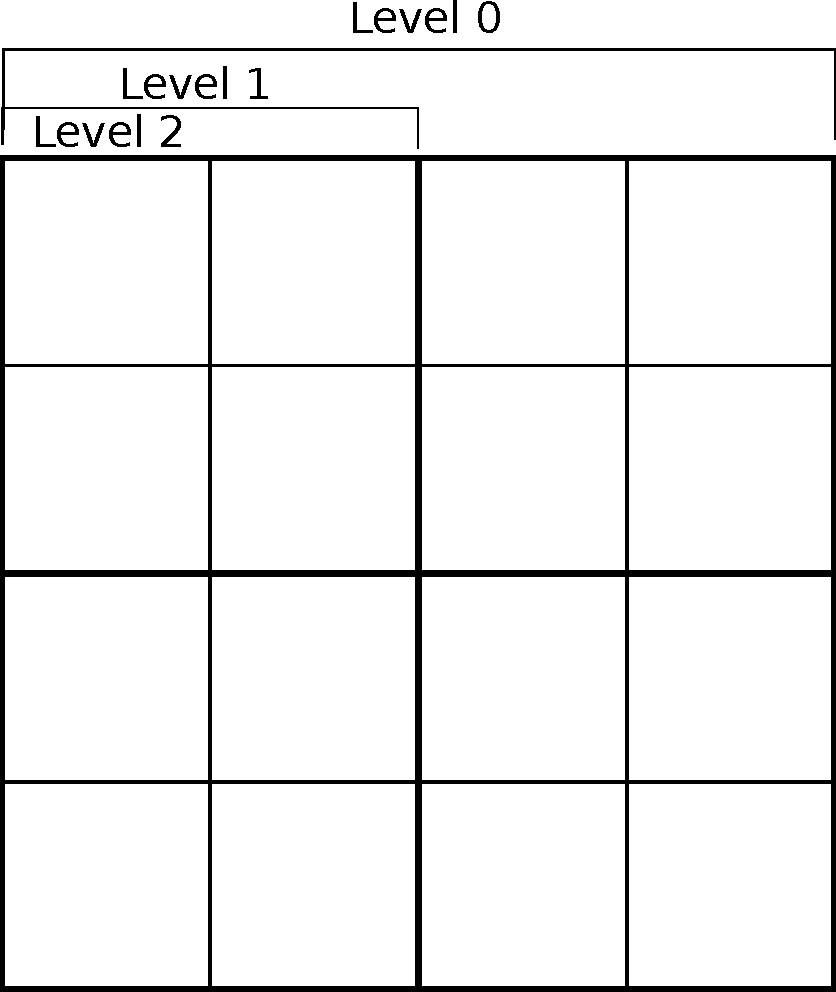
\includegraphics[width=0.35\textwidth]{figures/fma_mesh.pdf} \ecen
\caption{A simulation cell, with meshes up to level 2 displayed, giving $2^n = 2^2 = 4$ boxes per side}
\end{figure}

\subsection{Mathematical description}
\subsubsection{Potential and the multipole expansion approximation}
We describe the potential at a point $x_0 \in \mathbb{C}$ from the charge $q$ at $x \in \mathbb{C}$ by
\begin{equation}
\phi_{x_0} = -q\text{log}{|x - x_0|}
\label{eq:potential}
\end{equation}
A multipole expansion for this function is derived in \cite{greengard:315}. Suppose that $m$ charges of strength $\{q_i,i=1,...,m\}$ are located at points $\{z_i, i=1,...,m\}$, with $|z_i| < r$. Then for any $z \in \mathbb{C}$ with $|z| > r$, the potential $\phi(z)$ is given by
\begin{equation}
\phi(z) = Q \text{log}(z) + \sum_{k=1} ^{\infty} \frac{a_k}{z^k}
\label{eq:multipole_expansion}
\end{equation}
Where
\begin{equation}
Q = \sum_{i=1} ^m q_i 
\hspace{0.5cm} \text{and} \hspace{0.5cm}
a_k = \sum_{i=1} ^m \frac{-q_i z^k _i}{k}
\end{equation}
While this is exact for an infinite sum of terms, we can truncate the series at term $p$, and if $p$ is large enough, this approximation is close to the actual potential $\phi(z)$. A description of how close can be found in \cite{greengard:315}
\subsubsection{Shifting multipole expansions}
A multipole expansion's center may be shifted, which is necessary for the \fma. Suppose that
\begin{equation}
\phi(z) = a_0 \text{log}(z-z_0) + \sum_{k=1} ^{\infty} \frac{a_k}{(z-z_0)^k}
\label{eq:pre_shift_multipole}
\end{equation}
Describes a multipole expansion which is centered on $z_0$. We can then shift this multipole expansion to be centered at the origin,
\begin{equation}
\phi(z) = a_0 \text{log}(z) + \sum_{l=1} ^{\infty} \frac{b_l}{z^l}
\label{eq:shifted_multipole}
\end{equation}
Where
\begin{equation}
b_l = \left(\sum_{k=1} ^l a_k z_0^{l-k} \binom{l-1}{k-1} - \frac{a_0 z_0^l}{l} \right)
\label{eq:b_descr}
\end{equation}
Note that this procedure of shifting to the origin is equivalent to shifting from any point $a$ to point $b$, if we treaet point $b$ as the origin, and $a-b$ as our previous multipole expansion center.
\subsubsection{Local expansions}
We can find a local expansion about the origin due to a set of charges within radius $R$ of $z_0$, with $|z_0| > (c+1)R, \hs c > 1$. This local expansion is based on the multipole expansion at the same point.
\begin{equation}
\phi(z) = \sum _{l=0} ^{\infty} b_l * z^l
\label{local_expansion}
\end{equation}
Where
\begin{equation}
b_0 = \sum_{k=1} ^{\infty} \frac{a^k}{z^k_0} (-1)^k + a_0 \log(-z_0)
\label{where_local_expansion}
\end{equation}


\subsection{The algorithm}
The basic flow of the algorithm is given below\\
%%%%%PSEUDOCODE%%%%%%%%%
\begin{algorithm}[H]
\SetLine
\KwData{level-count: the number of mesh levels we create}
\For{i=0 to level-count}{Initialise mesh[i]}
\end{algorithm}

\subsection{The implementation}
\subsection{Analysis of the implementation}

\chapter{Comparison of the algorithms}
\label{chap:compare}
\chapter{Discussion}

\bibliographystyle{plain}	
\bibliography{references}	

\end{document}
